
%(BEGIN_QUESTION)
% Copyright 2009, Tony R. Kuphaldt, released under the Creative Commons Attribution License (v 1.0)
% This means you may do almost anything with this work of mine, so long as you give me proper credit

Determine the voltages registered by a voltmeter between the following points in this circuit.  Be sure to note whether the voltmeter's indication will be a positive value or a negative value in each case:

$$\includegraphics[width=15.5cm]{i02522x01.eps}$$

$V_A = \hbox{\underbar{ \hskip 20pt}}$ (red lead on {\bf A}, black lead on ground)

\vskip 5pt

$V_B = \hbox{\underbar{ \hskip 20pt}}$ (red lead on {\bf B}, black lead on ground)

\vskip 5pt

$V_C = \hbox{\underbar{ \hskip 20pt}}$ (red lead on {\bf C}, black lead on ground)

\vskip 5pt

$V_D = \hbox{\underbar{ \hskip 20pt}}$ (red lead on {\bf D}, black lead on ground)

\vskip 20pt

$V_{AC} = \hbox{\underbar{ \hskip 20pt}}$ (red lead on {\bf A}, black lead on {\bf C})

\vskip 5pt

$V_{DB} = \hbox{\underbar{ \hskip 20pt}}$ (red lead on {\bf D}, black lead on {\bf B})

\vskip 5pt

$V_{BA} = \hbox{\underbar{ \hskip 20pt}}$ (red lead on {\bf B}, black lead on {\bf A})

\vskip 5pt

$V_{BC} = \hbox{\underbar{ \hskip 20pt}}$ (red lead on {\bf B}, black lead on {\bf C})

\vskip 5pt

$V_{CD} = \hbox{\underbar{ \hskip 20pt}}$ (red lead on {\bf C}, black lead on {\bf D})

\vfil 

\underbar{file i02522}
\eject
%(END_QUESTION)





%(BEGIN_ANSWER)

This is a graded question -- no answers or hints given!

%(END_ANSWER)





%(BEGIN_NOTES)

The most important principle to bear in mind with this problem is the fact that {\it voltage is a relative quantity, always measured \underbar{between two points}}.  Consider the black test lead of a voltmeter as the ``reference'' or ``starting'' point, and the red test lead as the ``test'' or ``destination'' point.  Thus, a positively-signed voltmeter reading reflects a increase in electrical potential from the black lead to the red lead.  A negatively-signed voltmeter reading, conversely, reflects a decrease in electric potential from the black lead to the red lead.

\vskip 10pt

Electric potential is analgous to {\it height}, with ``ground'' referring to some commonly-established elevation of reference.  If we place the black test lead on point {\bf C} (-11 volts with reference to ground potential) it is analogous to placing the tip of a tape measure at the bottom of a hole 11 feet below ground level.  If we then place the red test lead on point {\bf A} (+20 volts with reference to ground potential) it is analogous to stretching the other end of the tape measure to the top of a hill 20 feet above ground level.  The vertical distance separating the bottom of an 11-foot hole and a 20-foot hill, is of course 31 feet.  To be more precise, the elevation change from the bottom of that hole to the top of that hill will be +31 feet, an {\it increase} in elevation.  If we were to reverse the leads between points (starting at {\bf A} and ending at {\bf C}), it would be a {\it decrease} in elevation (-31 feet, or -31 volts in the circuit).

\vskip 10pt

$V_A = \hbox{\underbar{ +20 volts}}$ (red lead on {\bf A}, black lead on ground)

\vskip 5pt

$V_B = \hbox{\underbar{ +5 volts}}$ (red lead on {\bf B}, black lead on ground)

\vskip 5pt

$V_C = \hbox{\underbar{ $-11$ volts}}$ (red lead on {\bf C}, black lead on ground)

\vskip 5pt

$V_D = \hbox{\underbar{ $-8$ volts}}$ (red lead on {\bf D}, black lead on ground)

\vskip 20pt

\goodbreak

$V_{AC} = \hbox{\underbar{ +31 volts}}$ (red lead on {\bf A}, black lead on {\bf C})

\vskip 5pt

$V_{DB} = \hbox{\underbar{ $-13$ volts}}$ (red lead on {\bf D}, black lead on {\bf B})

\vskip 5pt

$V_{BA} = \hbox{\underbar{ $-15$ volts}}$ (red lead on {\bf B}, black lead on {\bf A})

\vskip 5pt

$V_{BC} = \hbox{\underbar{ +16 volts}}$ (red lead on {\bf B}, black lead on {\bf C})

\vskip 5pt

$V_{CD} = \hbox{\underbar{ $-3$ volts}}$ (red lead on {\bf C}, black lead on {\bf D})



%INDEX% Electronics review: Kirchhoff's Voltage Law (KVL)

%(END_NOTES)


